% Planilla de mediciones del brazo XK-JS1-1 (versión imprimible)
% Misma información que la planilla en línea; se llena a mano en la planta.
% Compilar en esta carpeta:  latexmk -pdf planilla_mediciones.tex
\documentclass[10pt]{article}
\usepackage[landscape,letterpaper,margin=1.4cm,top=1.6cm,bottom=1.5cm]{geometry}
\usepackage[spanish, es-nodecimaldot, mexico]{babel}
\usepackage[utf8]{inputenc}
\usepackage[light,condensed,math]{kurier}
\usepackage[T1]{fontenc}
\usepackage[table]{xcolor}
\usepackage{graphicx, longtable, array, booktabs, amssymb, textcomp}
\usepackage{fancyhdr, lastpage, titlesec, enumitem}
\usepackage{hyperref}
\hypersetup{colorlinks=true, linkcolor=black, urlcolor=blue}
\graphicspath{{./}{fotos/}}

\definecolor{cafe}{RGB}{128,64,0}
\definecolor{naranja}{RGB}{194,98,12}
\definecolor{grayblack}{RGB}{50,50,50}
\definecolor{fondo}{RGB}{248,244,238}

\pagestyle{fancy}
\fancyhf{}
\lhead{\small ETN-902, ETN-1034, ETN-1000 · UMSA}
\chead{\small PLANILLA DE MEDICIÓN · BRAZO XK-JS1-1}
\rhead{\small Gestión II/2026}
\rfoot{\small Pág. \thepage\ de \pageref{LastPage}}
\lfoot{\small Medido por: \rule{5cm}{0.4pt}\quad Fecha: \rule{3cm}{0.4pt}}
\renewcommand{\headrulewidth}{0.6pt}
\renewcommand{\footrulewidth}{0.6pt}
\titleformat{\section}{\color{cafe}\normalfont\large\bfseries}{}{0pt}{}
\titlespacing*{\section}{0pt}{6pt}{4pt}

\setlength{\tabcolsep}{4pt}
\renewcommand{\arraystretch}{1.55}
\newcolumntype{L}[1]{>{\raggedright\arraybackslash}p{#1}}
% Tabla de mediciones: N.º | Dato | Código | Valor hoy | Cómo medirlo | Valor medido | Notas
\newenvironment{medidas}{%
  \small
  \begin{longtable}{@{}L{0.9cm}L{5.0cm}L{2.3cm}L{2.7cm}L{6.4cm}>{\columncolor{fondo}}L{3.1cm}L{2.4cm}@{}}
  \toprule
  \textbf{N.º} & \textbf{Dato} & \textbf{Código} & \textbf{Valor usado hoy} & \textbf{Cómo medirlo} & \textbf{Valor medido} & \textbf{Notas}\\
  \midrule\endhead
  \bottomrule\endfoot}{\end{longtable}}
\newcommand{\cod}[1]{\texttt{\footnotesize #1}}
\newcommand{\cajita}{$\square$}

\begin{document}
\color{grayblack}

%======================================================================== portada / instrucciones
\begin{center}
{\large\bfseries UNIVERSIDAD MAYOR DE SAN ANDRÉS · INGENIERÍA ELECTRÓNICA}\\[2pt]
{\LARGE\bfseries\color{cafe} Planilla de medición del brazo XK-JS1-1}\\[2pt]
{\normalsize Datos para que el modelo 3D, la cinemática y la tabla de pulsos dejen de depender de supuestos}
\end{center}

\section{Instrucciones}
\begin{minipage}[t]{0.47\textwidth}
\begin{itemize}[leftmargin=12pt, itemsep=1pt]
\item Llene la columna \textbf{Valor medido} (sombreada). \textbf{Valor usado hoy} es lo que tiene el modelo ahora
      (\cod{web/js/cinematica.js}). Si no puede medir algo, escriba el motivo en \textbf{Notas}.
\item \textbf{Herramientas:} calibrador de 150 mm o más, flexómetro, escuadra, nivel digital (app del celular),
      cinta de papel, marcador y celular para fotos.
\item \textbf{Unidades:} milímetros con un decimal si se puede; ángulos en grados.
\item \textbf{Seguridad:} para mover los carros a mano, apague el disyuntor (los motores con corriente bloquean el
      eje). Con el PLC, use la botonera en manual, a baja velocidad y con el auxiliar presente (Guía 4).
\item \textbf{Distancias entre centros:} siempre de centro de pasador a centro de pasador. Si solo puede medir
      bordes, mida también el diámetro del pasador (5.1).
\end{itemize}
\end{minipage}\hfill
\begin{minipage}[t]{0.47\textwidth}
\textbf{Convenciones del modelo (no cambiarlas al medir):}
\begin{itemize}[leftmargin=12pt, itemsep=1pt]
\item \textbf{Plano del brazo:} vista lateral con la garra a la derecha. $u$ horizontal hacia la garra; $h$ vertical
      desde la superficie de la mesa.
\item \textbf{Carro X ($s_X$):} 0 = bastidor atrás del todo (final trasero, \textbf{homing}); positivo hacia la garra.
\item \textbf{Carro Y ($s_Y$):} 0 = final inferior (\textbf{homing}: brazo abajo, bloque 1 adelante); positivo sube el
      brazo (el bloque 1 retrocede).
\item \textbf{$\theta$ base:} 0 = sensor inductivo activado; positivo antihorario visto desde arriba.
\item \textbf{Pieza n.º:} los números de las etiquetas pegadas en la planta (1 al 18), los mismos de los bocetos.
\item \textbf{Códigos de las figuras:} cada etiqueta naranja de los esquemas (por ejemplo \textcolor{naranja}{\textbf{5.9 L9}})
      es el número de fila de estas tablas.
\end{itemize}
\end{minipage}

\vspace{4pt}
\begin{center}
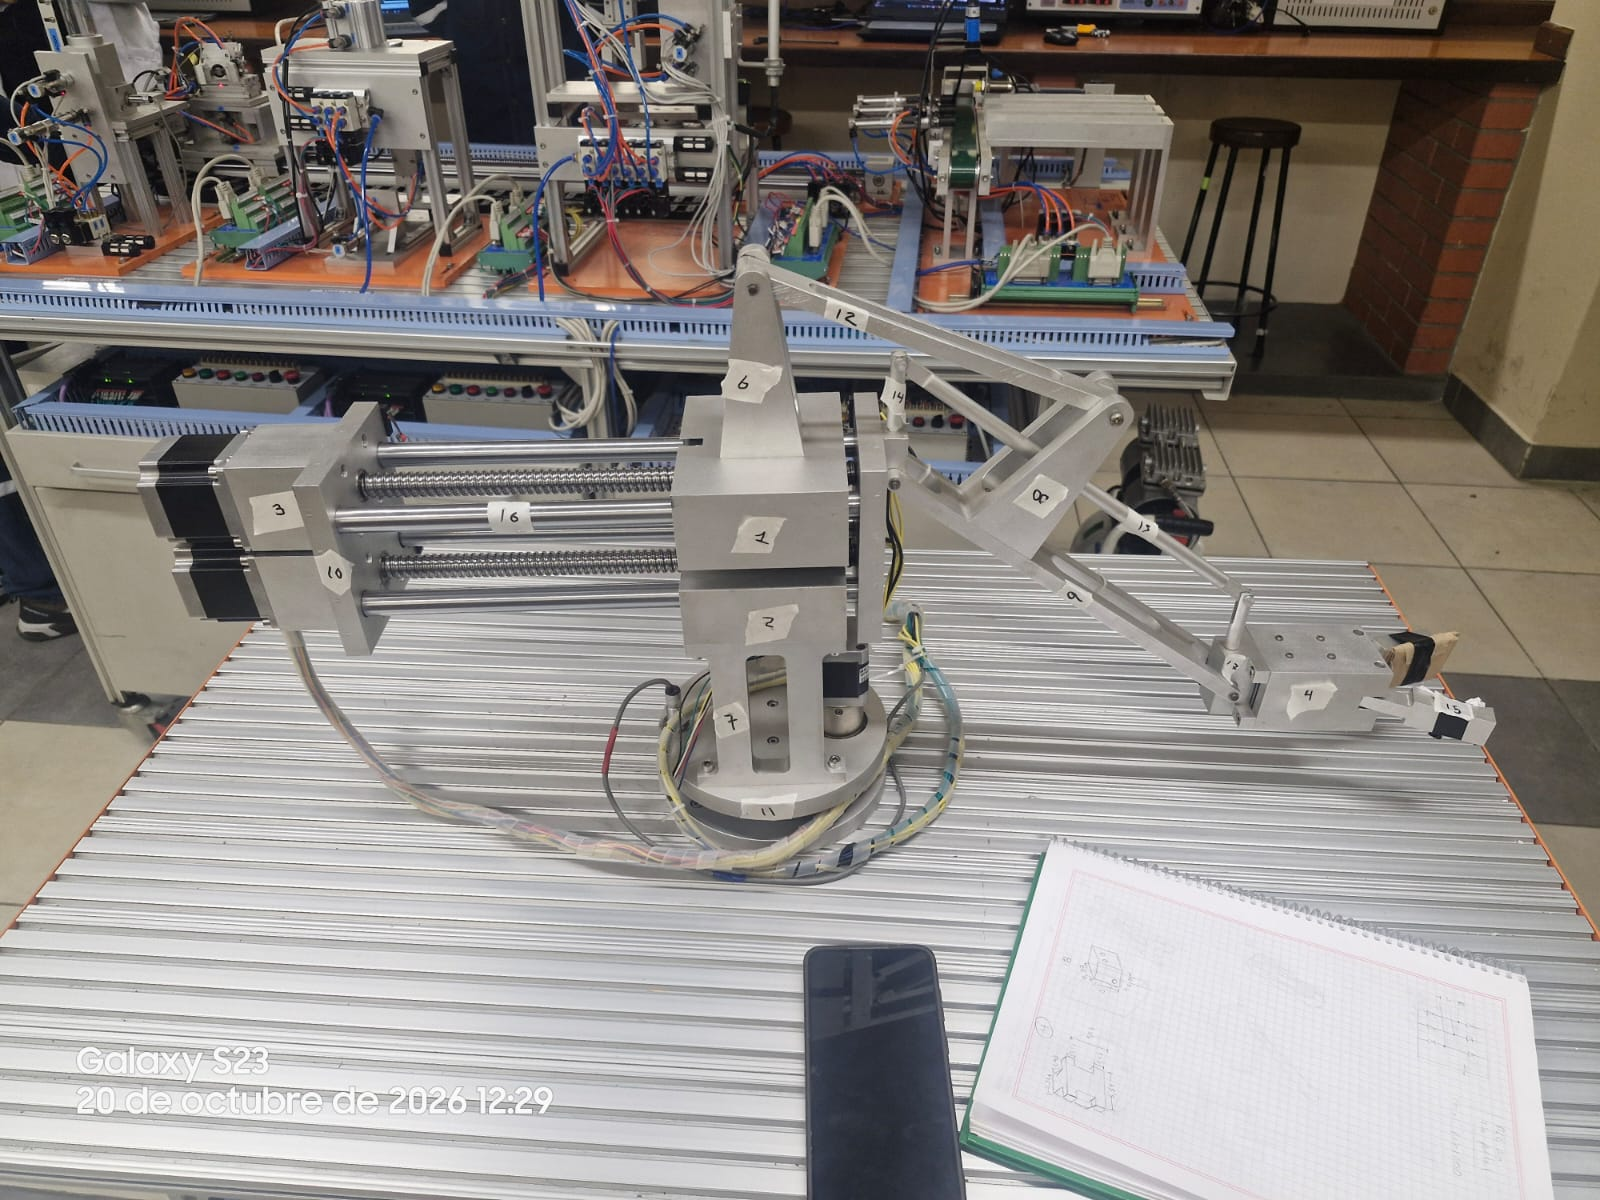
\includegraphics[height=0.40\textheight]{fotos/levantamiento_f13.jpg}\hspace{6pt}
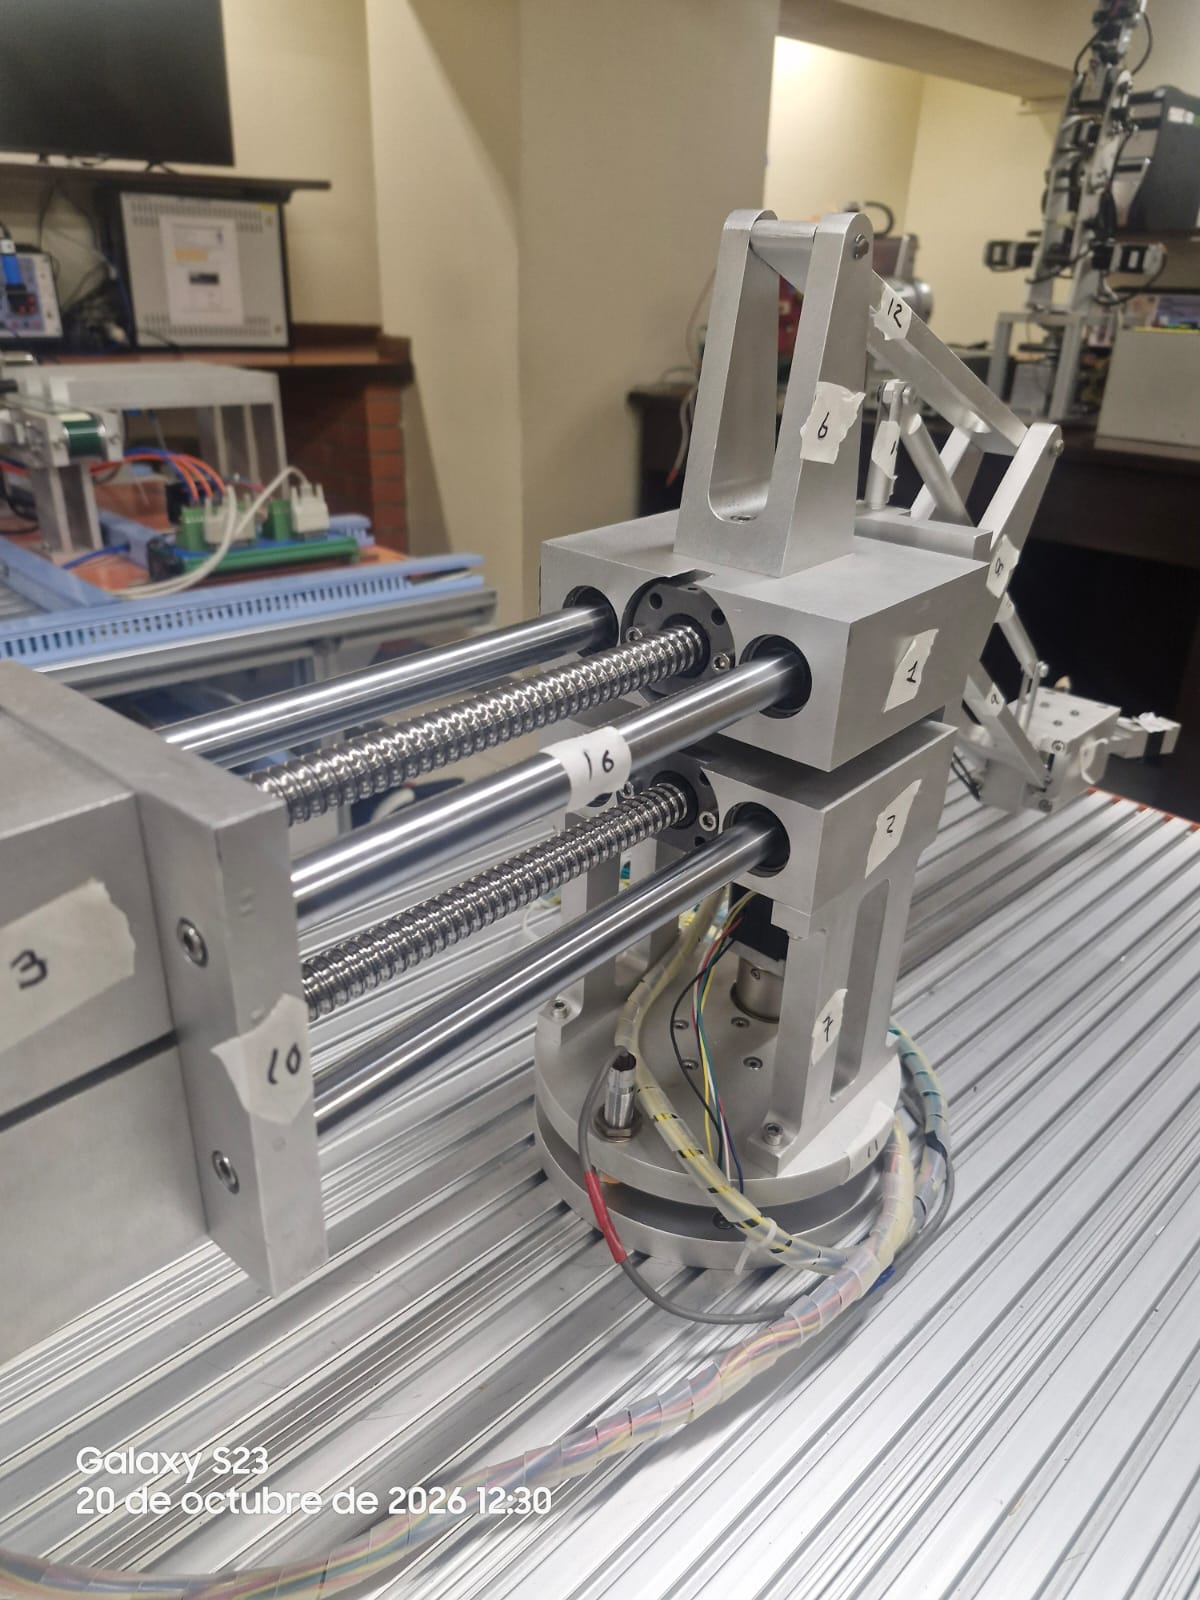
\includegraphics[height=0.40\textheight]{fotos/levantamiento_f12.jpg}\\[2pt]
{\small Piezas numeradas en la planta (fotos f13 y f12): 1 bloque carro Y, 2 bloque fijo, 3 adaptador de motor, 4 cuerpo de la
pinza, 5 y 10 placas, 6 y 8 escuadras, 7 columna, 9 brazo, 11 discos, 12 biela, 13 varilla, 14 postes, 15 dedos, 16 guías.}
\end{center}

\newpage
\begin{center}
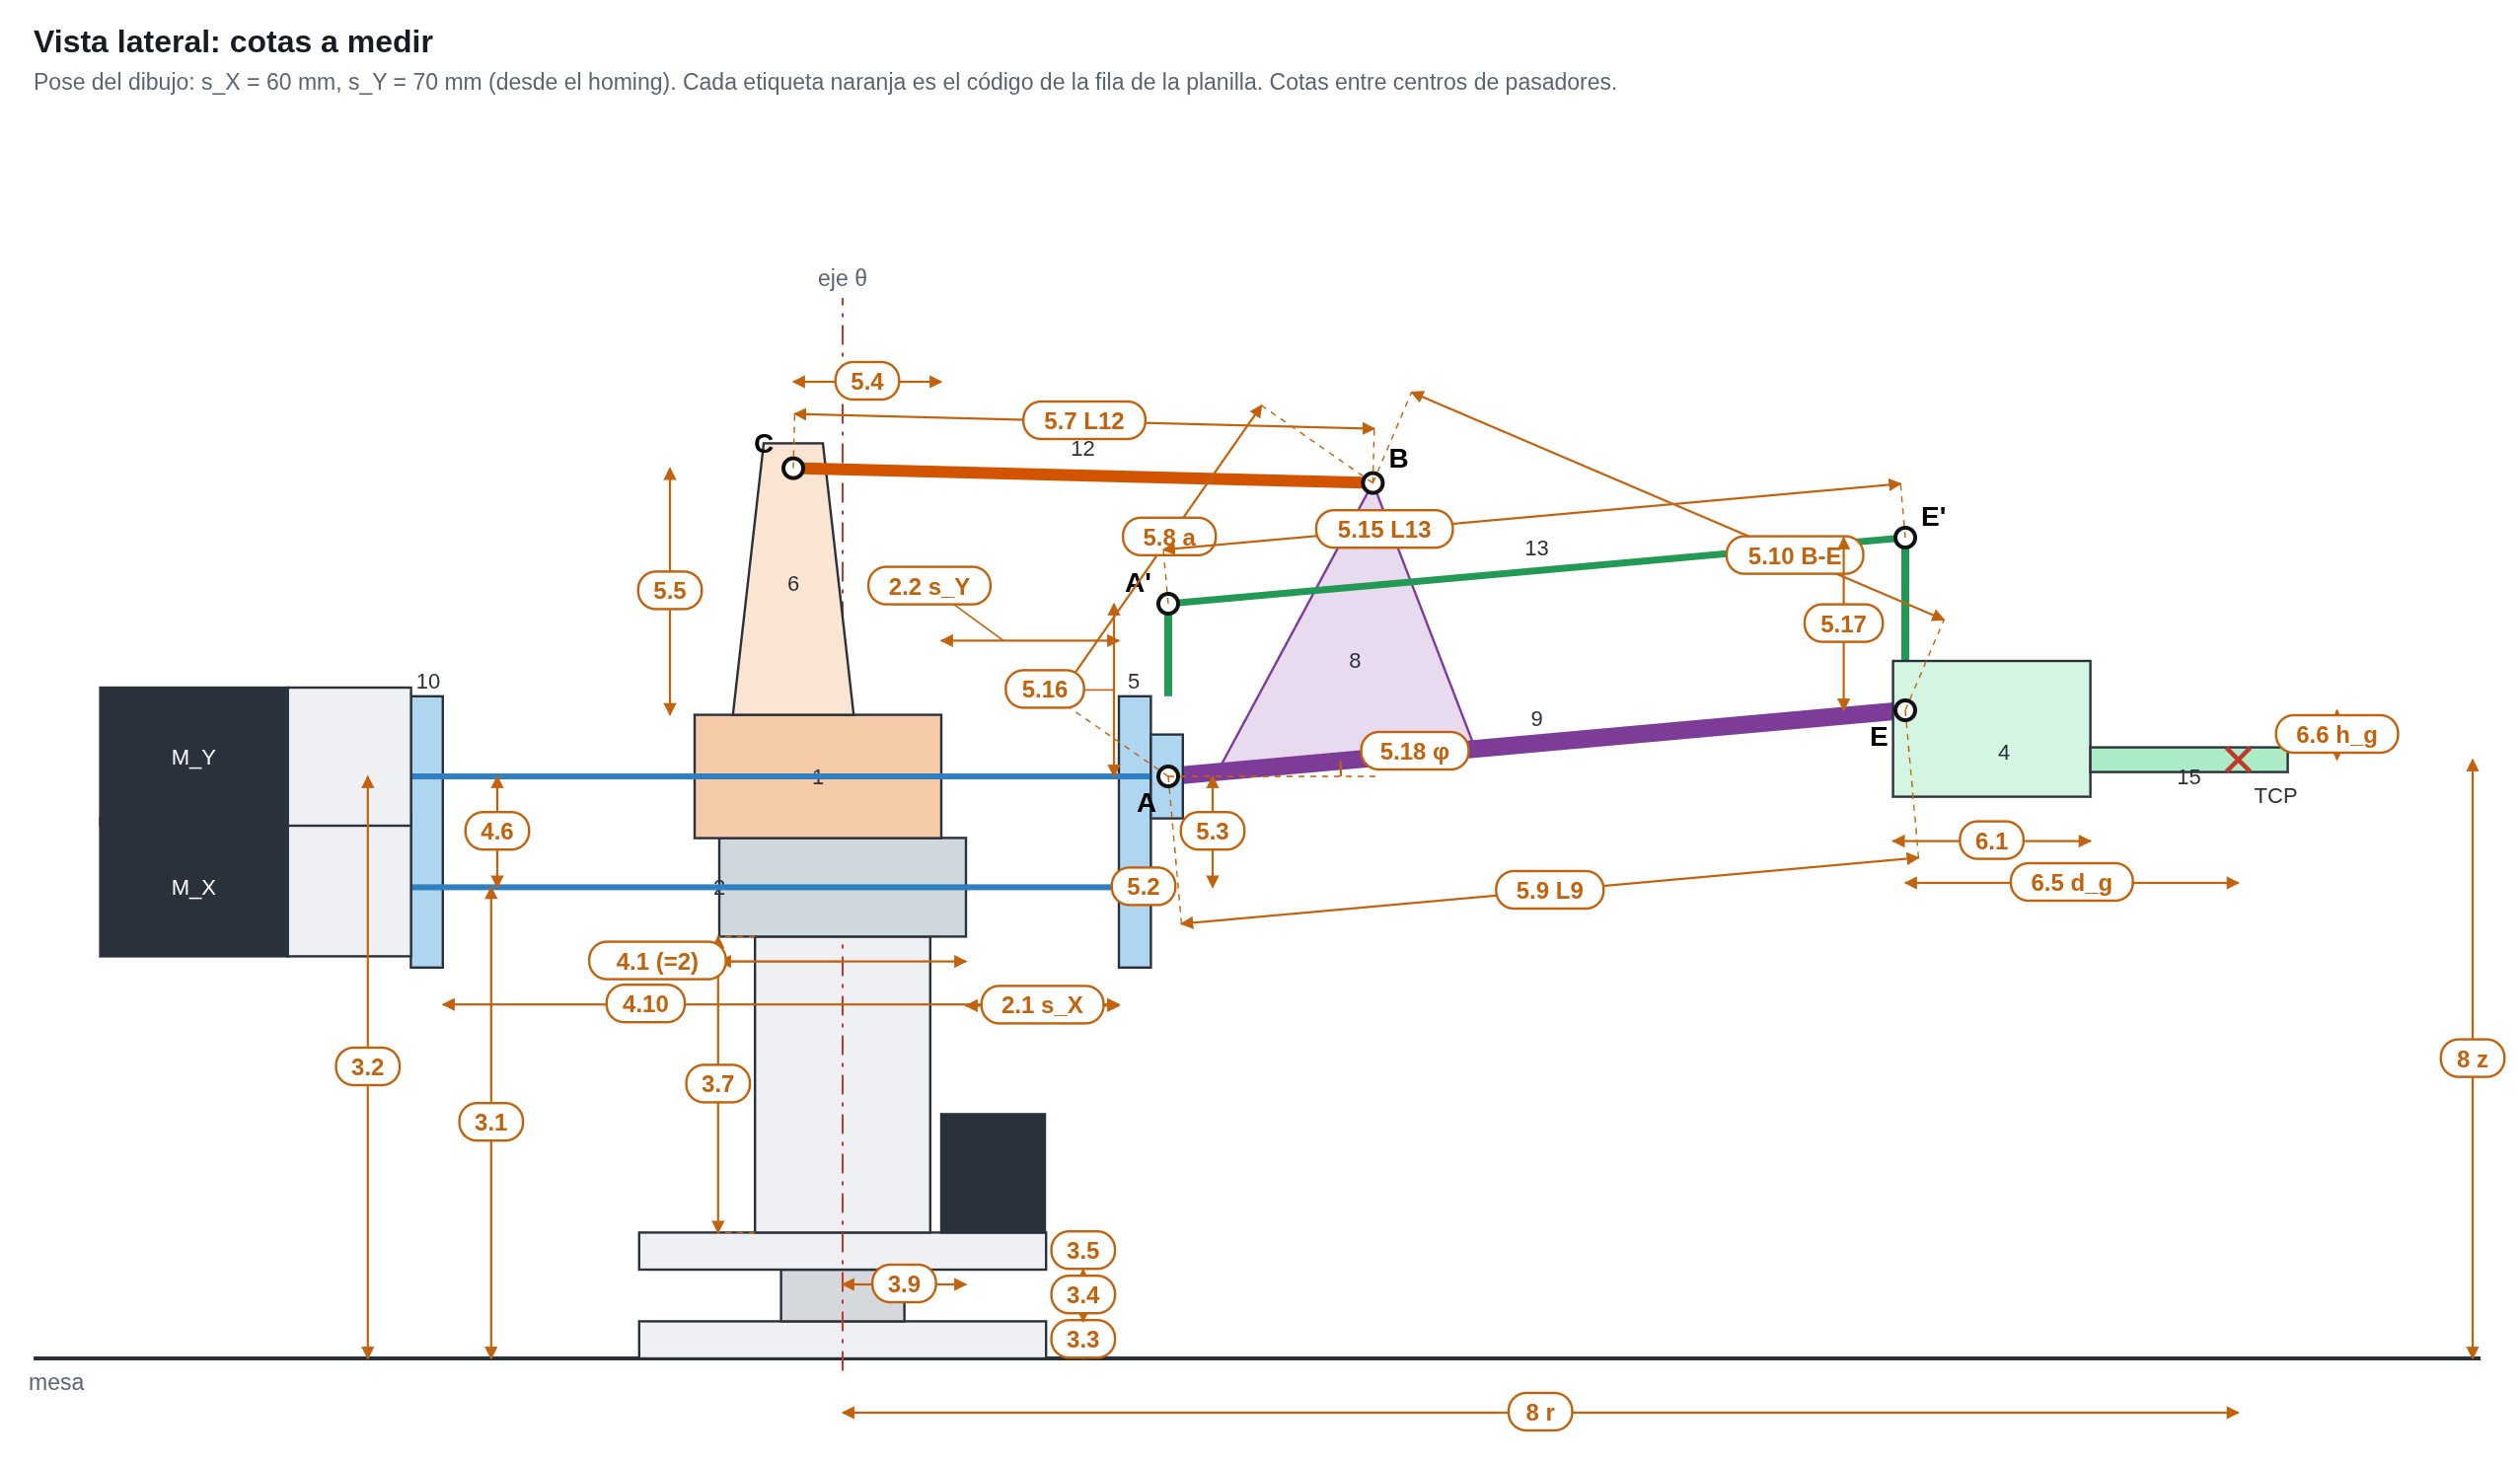
\includegraphics[width=\textwidth,height=0.86\textheight,keepaspectratio]{esquema_medidas_lateral.png}
\end{center}
\newpage
\begin{center}
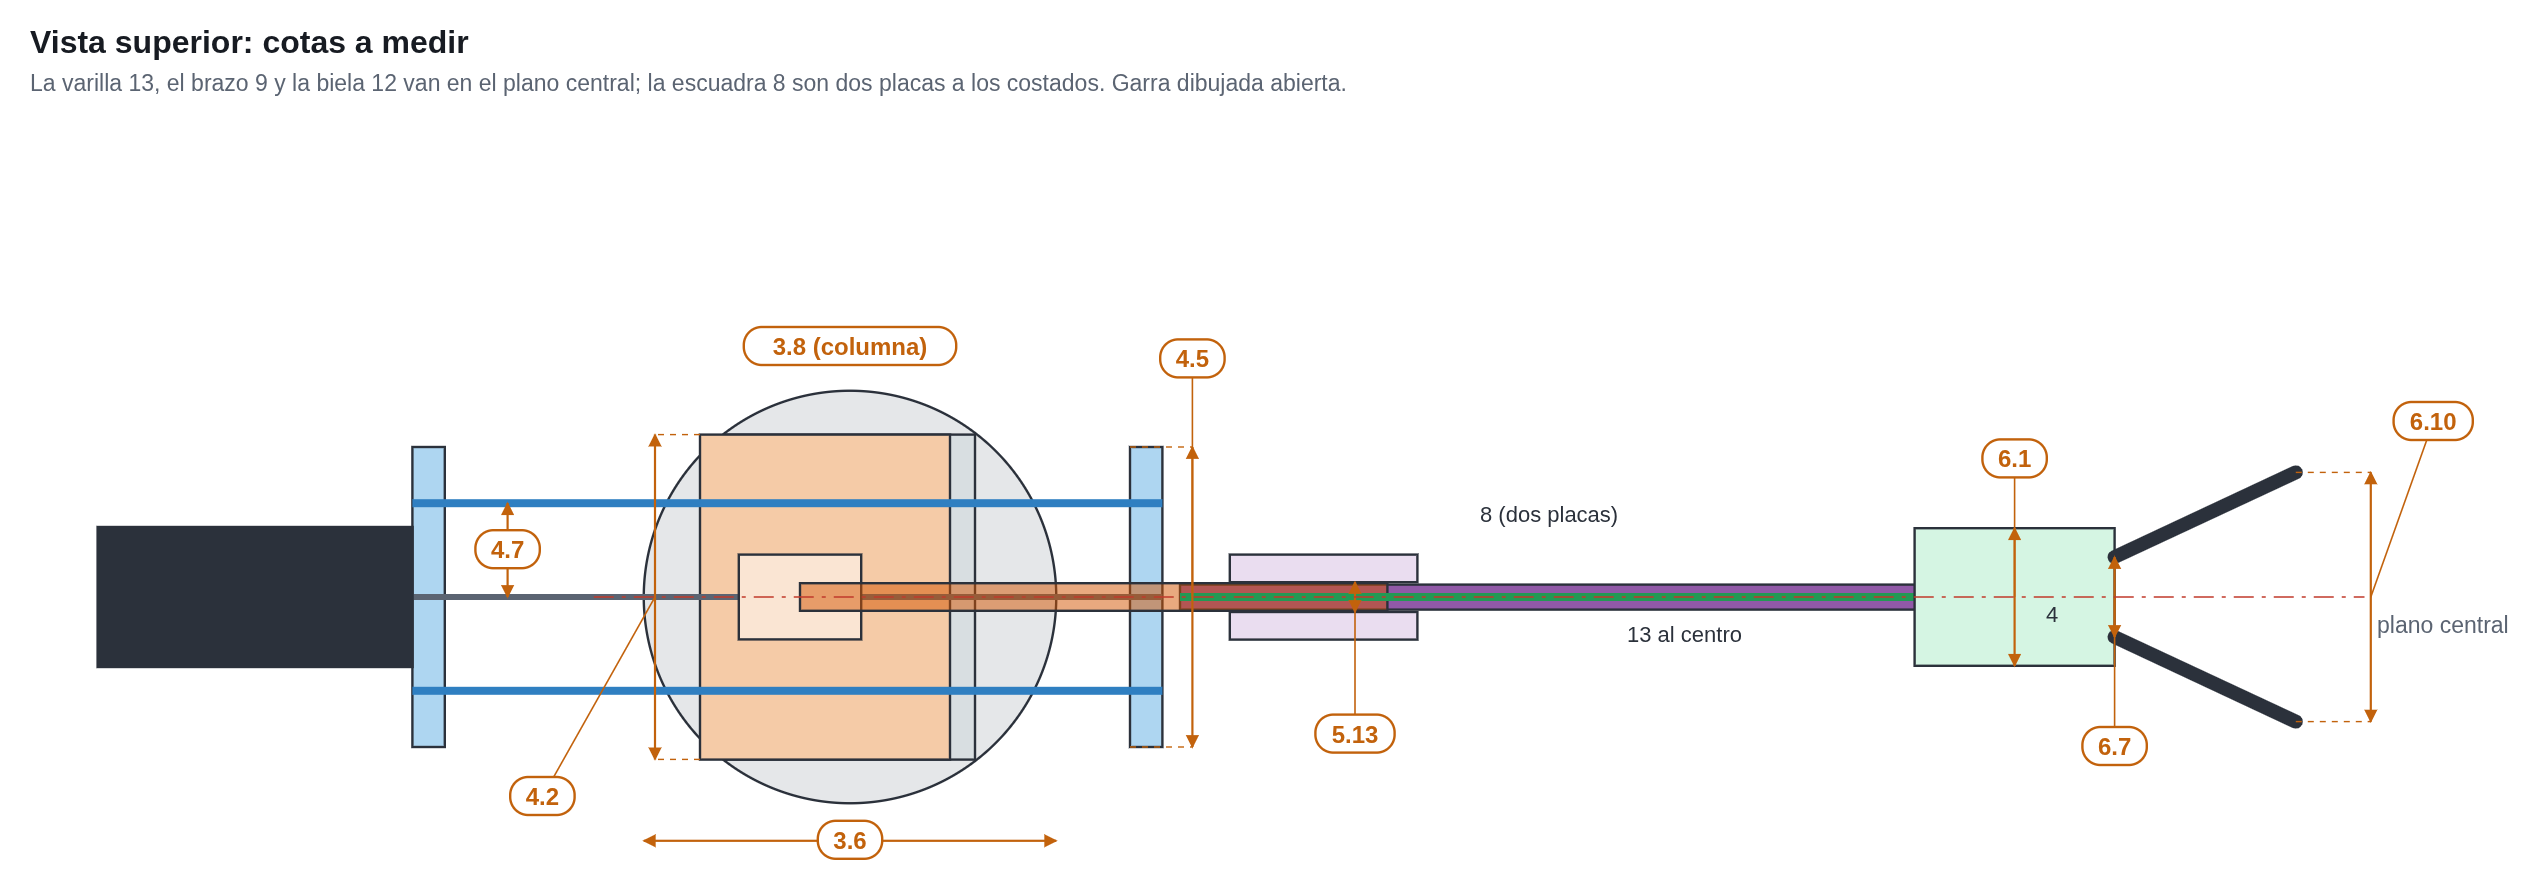
\includegraphics[width=\textwidth]{esquema_medidas_superior.png}\\[8pt]
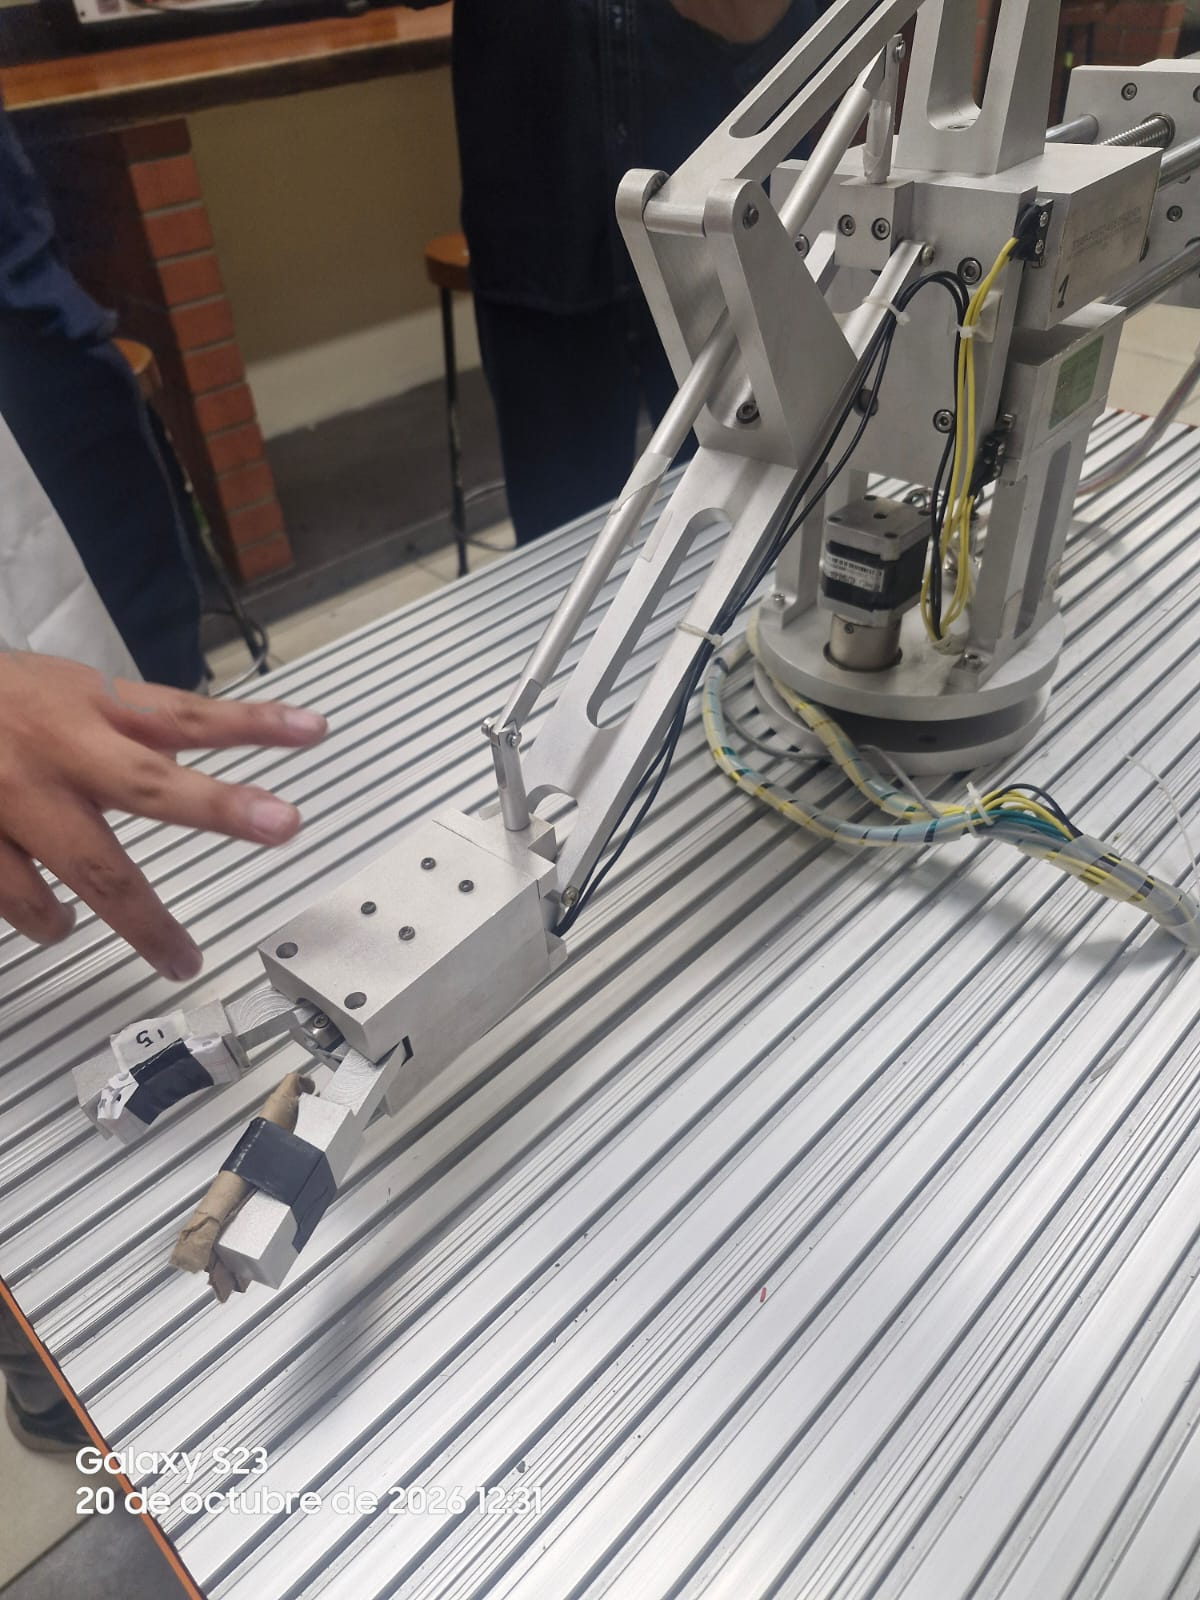
\includegraphics[height=0.36\textheight]{fotos/levantamiento_f18.jpg}\hspace{6pt}
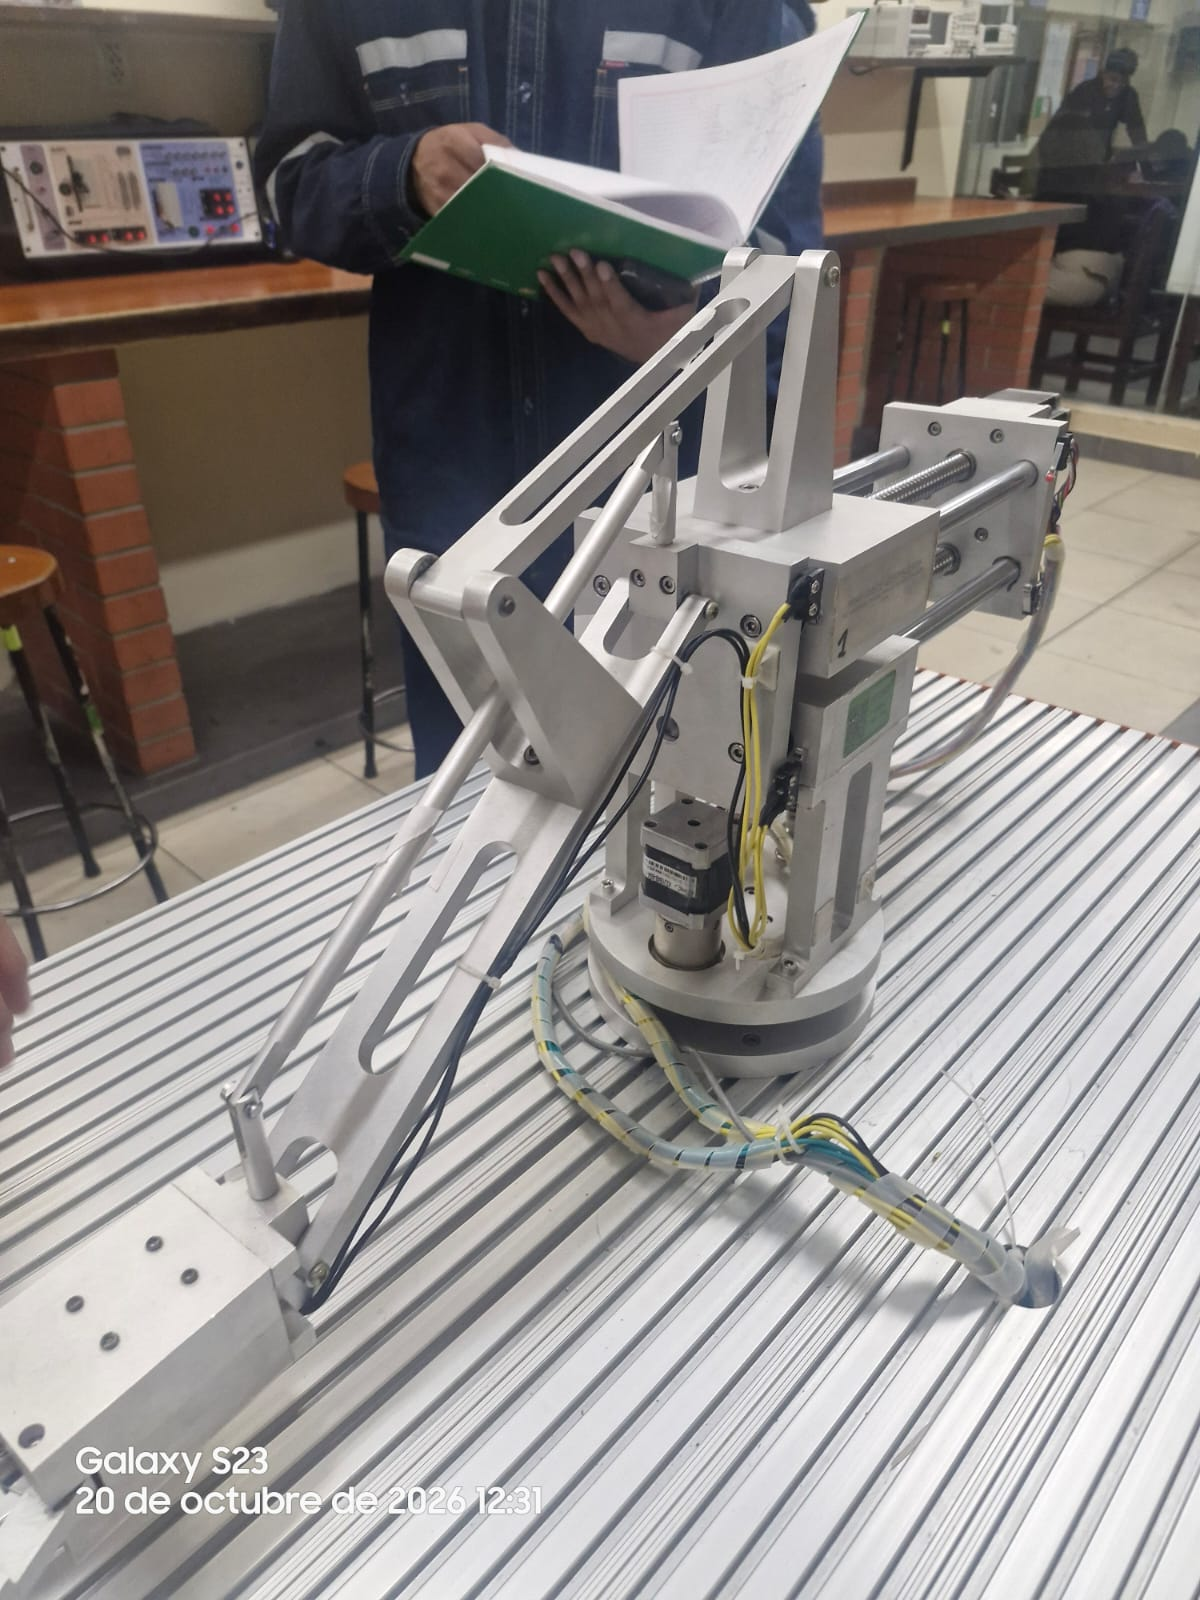
\includegraphics[height=0.36\textheight]{fotos/levantamiento_f19.jpg}\\[2pt]
{\small Pinza con sus dos dedos horizontales (f18) y vista frontal del mecanismo (f19).}
\end{center}

%======================================================================== 1
\newpage
\section{1. Transmisión y electrónica (prioridad alta)}
Convierten pulsos del PLC en milímetros y grados: un error aquí escala todas las posiciones. Hoy: 5 mm/rev, 1600 pulsos/rev, reducción 5:1.
\begin{medidas}
1.1 & Paso del husillo X (inferior) & \cod{pasoHusillo} & 5 mm/rev & Motores sin corriente. Marque el acople con cinta, gire el husillo 10 vueltas y mida cuánto avanzó el bastidor; paso = avance / 10. & & \\
1.2 & Paso del husillo Y (superior) & \cod{pasoHusillo} & 5 mm/rev & Igual que 1.1, midiendo el avance del bloque 1. & & \\
1.3 & Diámetro exterior del husillo & -- & 16--21 mm & Calibrador sobre las crestas de la rosca. & & \\
1.4 & Grabado de la tuerca de bolas & -- & SFU1605 (supuesto) & Leer el grabado de la brida (SFU1605, SFU2005\ldots). Foto. & & \\
1.5 & Pulsos por vuelta, driver X (2M542) & \cod{micropasosXY} & 1600 (SW4--SW7 = 0 0 1 1) & Foto de los DIP. Anote SW1 a SW8 (ON = 1). & SW1--8: & \\
1.6 & Pulsos por vuelta, driver Y (2M542) & \cod{micropasosXY} & 1600 & Igual que 1.5 en el driver Y. & SW1--8: & \\
1.7 & Pulsos por vuelta, driver base (2M530) & \cod{micropasosZ} & 1600 & Igual que 1.5 en el driver de la base. & SW1--8: & \\
1.8 & Corriente configurada, drivers X / Y / base & -- & sin dato & De los mismos DIP (SW1--SW3). & & \\
1.9 & Dientes del piñón del motor de la base & \cod{reduccionBase} & -- & Contar dientes (si no se ve, usar 1.11). & & \\
1.10 & Dientes de la corona de la base & \cod{reduccionBase} & -- & Contar dientes; reducción = corona / piñón. & & \\
1.11 & Reducción de la base (método alternativo) & \cod{reduccionBase} & 5:1 & Enviar N pulsos a Q0.0 (ej. 8000) y medir el ángulo girado; reducción = N · 360 / (pulsos/rev · ángulo). & & \\
1.12 & DIR X = 1 mueve el bastidor hacia\ldots & Q0.3 & la garra (supuesto) & Mover con la botonera y mirar el LED de Q0.3. & \cajita\ garra\quad \cajita\ motores & \\
1.13 & DIR Y = 1 mueve el bloque 1 hacia\ldots & Q0.4 & la garra (supuesto) & Igual, LED de Q0.4. & \cajita\ garra\quad \cajita\ motores & \\
1.14 & DIR base = 1 gira (visto desde arriba)\ldots & Q0.2 & antihorario (supuesto) & Igual, LED de Q0.2. & \cajita\ antihor.\quad \cajita\ horario & \\
1.15 & Frecuencia de pulsos del programa (manual / automático) & \cod{fMaxPTO} & 20 kHz máx. & Proyecto Micro/WIN (asistente de posición o SMW68/SMW78). & & \\
\end{medidas}

%======================================================================== 2
\section{2. Recorridos y referencias (prioridad alta)}
Fijan los límites de los deslizadores, el homing y el espacio de trabajo. Hoy: carro X 0--120 mm (ficha del fabricante), carro Y 0--170 mm, base $\pm$175°.
\begin{medidas}
2.1 & Carrera útil del carro X entre sus finales de carrera & \cod{recorridoX} & 120 mm & Bastidor al final trasero: marque con cinta la placa 5 sobre el bloque 2; luego al delantero; mida entre marcas. & & \\
2.2 & Carrera útil del carro Y entre sus finales de carrera & \cod{recorridoY} & 170 mm & Igual, marcando la cara delantera del bloque 1 sobre una guía superior. & & \\
2.3 & Pulsos de X entre finales (si se puede con el PLC) & -- & 38 400 (calc.) & Contador del programa al ir de un final al otro. Verifica 1.1 y 1.5. & & \\
2.4 & Pulsos de Y entre finales & -- & 54 400 (calc.) & Igual que 2.3. & & \\
2.5 & Holgura bloque 2 -- placa 5 con X en su final trasero (homing) & \cod{holgura} & 2 mm & Calibrador entre la cara delantera del bloque 2 y la cara interior de la placa 5. & & \\
2.6 & Holgura bloque 1 -- placa 5 con Y en su final inferior (homing) & \cod{holgura} & 2 mm & Calibrador entre la cara delantera del bloque 1 y la cara interior de la placa 5. & & \\
2.7 & Final que usa el homing de X & -- & trasero (I0.1), confirmado & -- & \checkmark\ confirmado & \\
2.8 & Final que usa el homing de Y & -- & inferior (I0.4), confirmado & -- & \checkmark\ confirmado & \\
2.9 & Giro máximo de la base hacia la izquierda desde el inductivo & \cod{thetaMax} & +175° & Girar despacio hasta que los cables queden tensos; medir con transportador. & & \\
2.10 & Giro máximo de la base hacia la derecha & \cod{thetaMin} & $-$175° & Igual que 2.9. & & \\
2.11 & Ancho angular de detección del inductivo & -- & $\pm$0.5° & Girar lento; anotar ángulo de entrada y de salida del LED del sensor. & & \\
2.12 & Hacia dónde apunta el brazo con $\theta$ = 0 & -- & eje largo de la mesa & Foto desde arriba con el inductivo activado. & & \\
\end{medidas}

%======================================================================== 3
\section{3. Base, columna y alturas}
La altura de los husillos decide la altura Z de la garra en todo el modelo. Hoy: 191 mm (inferior) y 236 mm (superior).
\begin{medidas}
3.1 & \textbf{Altura del eje del husillo inferior sobre la mesa} & suma de alturas & 191 mm & Escuadra apoyada en la mesa hasta el centro del husillo, en la cara del bloque 2. & & \\
3.2 & \textbf{Altura del eje del husillo superior sobre la mesa} & \cod{sepNiveles} & 236 mm & Igual, al centro del husillo superior en la cara del bloque 1. & & \\
3.3 & Espesor del disco inferior (fijo) & \cod{hDiscoInf} & 15 mm & Calibrador. & & \\
3.4 & Separación entre discos & \cod{hEntreDiscos} & 21 mm & Calibrador por el costado. & & \\
3.5 & Espesor del disco superior (gira) & \cod{hDiscoSup} & 15 mm & Calibrador. & & \\
3.6 & Diámetro de los discos & \cod{rDisco} & Ø 165 mm & Calibrador o flexómetro. & & \\
3.7 & Altura de la columna 7 & \cod{hColumna} & 120 mm & Del disco superior a la cara inferior del bloque 2. & & \\
3.8 & Ancho × profundidad de la columna 7 & -- & 100 × 71 mm & Calibrador; indique cuál lado es paralelo a las guías. & & \\
3.9 & Eje de giro a la cara delantera del bloque 2 & \cod{largoBloque}/2 & 50 mm & Del centro del disco a la cara del bloque 2 que mira a la garra. & & \\
3.10 & Desplazamiento lateral del plano del brazo respecto al eje de giro & -- & 0 mm & Desde arriba: ¿el husillo pasa sobre el centro del disco? & & \\
3.11 & Posición del NEMA 17 sobre el disco & -- & delante de la columna & Foto desde arriba. & & \\
3.12 & Posición del sensor inductivo y de su leva & -- & sobre el disco superior & Foto; en qué disco va el sensor y en cuál la leva. & & \\
\end{medidas}

%======================================================================== 4
\section{4. Bastidor, bloques, placas, guías y motores}
Definen la carrera máxima posible y la forma del modelo 3D; casi todas están en los bocetos y solo hay que confirmarlas.
\begin{medidas}
4.1 & Bloques 1 y 2: largo a lo largo de las guías & \cod{largoBloque} & 100 mm & Calibrador. & & \\
4.2 & Bloque 1: ancho (lateral) × alto & \cod{anchoBloque}, \cod{hBloque1} & 130 × 50 mm & Calibrador. & & \\
4.3 & Bloque 2: largo × ancho × alto & \cod{hBloque2} & 100 × 130 × 40 mm & Calibrador. & & \\
4.4 & Desfase entre bloques 1 y 2 en el homing & -- & variable & Anote $s_X$, $s_Y$ y el desfase. & & \\
4.5 & Placas 5 y 10: ancho (lateral) × alto × espesor & \cod{anchoPlaca}, \cod{altoPlaca} & 120 × 110 × 13 mm & Calibrador. & & \\
4.6 & Separación vertical entre ejes de husillos & \cod{sepNiveles} & 45 mm & Centro a centro en la placa. & & \\
4.7 & Separación lateral guía -- husillo (centro a centro) & \cod{zGuias} & 37.5 mm & Centro a centro en la placa, a cada lado. & & \\
4.8 & Borde inferior de la placa al eje del husillo inferior & -- & 32.5 mm & Calibrador. & & \\
4.9 & Guías 16: longitud total y diámetro & \cod{largoGuias} & 300 × Ø16 mm & Flexómetro y calibrador. & & \\
4.10 & Distancia libre entre caras interiores de las placas 5 y 10 & -- & 274 mm & Flexómetro entre placas. & & \\
4.11 & Largo del adaptador del motor (pieza 3) & -- & 50 mm & Calibrador. & & \\
4.12 & Largo del cuerpo del motor NEMA 23 & -- & 76 mm & Calibrador. & & \\
4.13 & ¿Qué motor está arriba: X o Y? & -- & arriba Y (manual) & Seguir el cable hasta el driver rotulado. & \cajita\ X\quad \cajita\ Y & \\
4.14 & Posición de cada final de carrera (placa, nivel, lado) & -- & 2 por placa & Foto de cada placa. & & \\
\end{medidas}

%======================================================================== 5
\section{5. Mecanismo de bielas (prioridad alta)}
Definen cuánto sube y baja la garra con el carro Y; hoy casi todas son estimadas de fotos. Pivotes: \textbf{A} brazo 9 en la placa 5, \textbf{A'} varilla 13
sobre la placa 5, \textbf{B} punta de la escuadra 8, \textbf{C} punta de la escuadra 6, \textbf{E} brazo 9 en la pinza, \textbf{E'} varilla 13 en la pinza.
El ángulo $\beta$ se calcula con 5.8, 5.9 y 5.10 (no hace falta transportador).
\begin{medidas}
5.1 & Diámetro de los pasadores (A, B, C, E, A', E') & -- & Ø 9 mm & Calibrador; sirve para pasar de bordes a centros. & & \\
5.2 & \textbf{A}: de la cara interior de la placa 5 al centro de A & \cod{uA} & 20 mm & Calibrador desde la cara que mira a los bloques, hacia la garra. & & \\
5.3 & \textbf{A}: altura sobre el eje del husillo inferior & \cod{dhA} & 45 mm & Escuadra; o altura de A sobre la mesa menos 3.1. & & \\
5.4 & \textbf{C}: de la cara delantera del bloque 1 al centro de C (negativo si está detrás) & \cod{uCBloque} & $-$60 mm & Calibrador o escuadra en la cara del bloque 1. & & \\
5.5 & \textbf{C}: altura sobre la cara superior del bloque 1 & \cod{hC}+\cod{dhC} & 100 mm & Calibrador desde la cara superior del bloque 1. & & \\
5.6 & Escuadra 6: alto, base, punta, espesor de placa, separación interior & -- & 110 / 49 / 24 / 11 / 12 mm & Calibrador; ¿pieza en U o dos placas? & & \\
5.7 & \textbf{L12}: biela 12, de C a B & \cod{L12} & 235 mm & Flexómetro o calibrador entre pasadores. & & \\
5.8 & \textbf{a}: de A a B (balancín 8 + 9) & \cod{a} & 145 mm & Calibrador entre pasadores. & & \\
5.9 & \textbf{L9}: brazo 9, de A a E & \cod{L9} & 300 mm & Flexómetro entre pasadores. & & \\
5.10 & De B a E & -- (da $\beta$) & 235 mm (calc.) & Flexómetro entre pasadores. & & \\
5.11 & $\beta$ = arccos((a² + L9² $-$ BE²) / (2·a·L9)) & \cod{beta} & 50° & Se calcula con 5.8, 5.9 y 5.10. & & \\
5.12 & Escuadra 8: distancias desde A de sus dos vértices sobre el brazo & -- & 20 y 125 mm & Flexómetro a lo largo del brazo. & & \\
5.13 & Separación interior entre las dos placas de la escuadra 8 & -- & 12 mm & Calibrador (por ahí pasa la varilla 13). & & \\
5.14 & Brazo 9: ancho, espesor, ¿una o dos placas? & -- & 46 × 10, una & Calibrador. & & \\
5.15 & \textbf{L13}: varilla 13, de A' a E' & \cod{L9} & 300 mm & Flexómetro. Si difiere de 5.9, anote la diferencia. & & \\
5.16 & \textbf{L14}: poste trasero, de A a A' & \cod{L14} & 70 mm & Calibrador. ¿A' está justo sobre A? & & \\
5.17 & \textbf{L14}: poste delantero, de E a E' & \cod{L14} & 70 mm & Calibrador. Debe ser igual a 5.16. & & \\
5.18 & Ángulo del brazo 9 con $s_X$ = 0 y Y en su final inferior (homing) & -- & $-$32.6° (calc.) & Nivel digital del celular sobre el brazo 9. & & \\
5.19 & Ángulo del brazo 9 con Y en su final superior & -- & +47° (calc.) & Igual que 5.18. & & \\
5.20 & Ángulo del brazo 9 con Y al centro de su carrera & -- & +12° ($s_Y$ = 85) & Igual; anote el $s_Y$ real. & & \\
\end{medidas}

%======================================================================== 6
\section{6. Pinza (garra)}
Definen dónde está el punto de trabajo (TCP: centro entre los bloques de agarre cerrados) respecto del pivote E, y cómo se mueven los dedos.
\begin{medidas}
6.1 & Cuerpo 4: largo × ancho (lateral) × alto & \cod{hCuerpoPinza} & 80 × 55 × 55 mm & Calibrador. & & \\
6.2 & Pivote E: distancia desde la cara trasera del cuerpo 4 & -- & 5 mm & Calibrador. & & \\
6.3 & Pivote E: distancia desde la cara inferior del cuerpo 4 & \cod{pinzaBajoE} & 35 mm & Calibrador. & & \\
6.4 & Poste delantero 14 sobre el cuerpo (desde atrás y desde el costado) & -- & sobre E, al centro & Calibrador. & & \\
6.5 & \textbf{d\_g}: horizontal de E al centro de los bloques de agarre & \cod{dg} & 135 mm & Flexómetro con la pinza horizontal y la garra cerrada. & & \\
6.6 & \textbf{h\_g}: cuánto más abajo que E está ese centro & \cod{hg} & 20 mm & Escuadra con la pinza horizontal. & & \\
6.7 & Pivotes de los dedos: distancia desde E y separación lateral & -- & 75 mm; 32 mm & Calibrador. & & \\
6.8 & Dedo: largo del pivote a la punta, ancho, espesor & -- & 80 × 16 × 10 mm & Calibrador. & & \\
6.9 & Bloque de agarre (con cinta): largo × ancho × alto & -- & 40 × 20 × 26 mm & Calibrador. & & \\
6.10 & Apertura máxima entre puntas (Q0.7 OFF) & -- & $\sim$55 mm ($\pm$25°) & Calibrador entre caras de agarre. Fabricante: 0--100 mm. & & \\
6.11 & Separación entre caras con la garra cerrada (Q0.7 ON) & -- & 0 mm & Calibrador; 0 si se tocan. & & \\
6.12 & Con Q0.7 = ON la garra\ldots & -- & cierra (manual) & Probar con S1 en modo manual. & \cajita\ cierra\quad \cajita\ abre & \\
6.13 & Altura mínima segura del TCP sobre la mesa & colisión & 15 mm & Bajar despacio el carro Y con $s_X$ a mitad y medir cuando la pinza casi toca. & & \\
\end{medidas}

%======================================================================== 7
\section{7. Mapa de E/S del PLC (confirmar en la planta)}
El manual y el README no coinciden en las entradas; mire el LED del PLC al accionar cada sensor o botón.
{\small
\begin{longtable}{@{}L{1.4cm}L{5.2cm}L{3.6cm}L{3.4cm}>{\columncolor{fondo}}L{6.2cm}L{3.6cm}@{}}
\toprule
\textbf{Punto} & \textbf{Según el manual (tabla 2-1)} & \textbf{README / Informe 1} & \textbf{Simulación} & \textbf{Qué hace en la planta} & \textbf{Notas}\\
\midrule\endhead
\bottomrule\endfoot
I0.0 & Sensor inductivo de la base & Final de carrera & Inductivo $\theta$ = 0 & & \\
I0.1 & Final X ``before'' & Final de carrera & Final X atrás & & \\
I0.2 & Final X ``after'' & Final de carrera & Final X adelante & & \\
I0.3 & Final Y arriba & Final de carrera & Final Y arriba & & \\
I0.4 & Final Y abajo & Botón QA & Final Y abajo & & \\
I0.5--I1.5 & Botonera (Auto, Reset, Start, Stop, S2--S7) & Botonera & -- & & \\
Q0.0 & Pulsos de la base (PTO) & Pulsos base & Pulsos base & & \\
Q0.1 & Pulsos X/Y compartidos (PTO) & no figura & PTO X/Y & & \\
Q0.2 & DIR base & DIR base & DIR base & & \\
Q0.3 & DIR X & DIR X & DIR X & & \\
Q0.4 & DIR Y & DIR Y & DIR Y & & \\
Q0.5 & ``X pulse'' (relé K1, Informe Lab 2) & Pulsos X & Relé K1 $\rightarrow$ X & & \\
Q0.6 & ``Y pulse'' (relé K2, Informe Lab 2) & Pulsos Y & Relé K2 $\rightarrow$ Y & & \\
Q0.7 & Garra (relé K3) & Garra & Garra & & \\
\end{longtable}}
\noindent\textbf{Pregunta clave:} con S4 (adelante) presionado, ¿qué LED parpadea? \cajita\ Q0.1\quad \cajita\ Q0.5\quad \cajita\ otro: \rule{3cm}{0.4pt}
(si es Q0.1, X e Y comparten el PTO y no pueden moverse a la vez).

%======================================================================== 8
\newpage
\section{8. Validación del modelo}
Haga homing (X atrás, Y abajo: ahí $s_X = s_Y = 0$ y los pulsos parten de cero), lleve los carros a cada posición y mida $r$ (horizontal, del centro del disco al
centro de los bloques de agarre) y $z$ (altura de ese centro sobre la mesa). Si no puede enviar pulsos, mida al menos las filas 1, 5, 21 y 25 moviendo a mano.
{\small\renewcommand{\arraystretch}{1.32}
\begin{longtable}{@{}rrrrrrr>{\columncolor{fondo}}p{2.6cm}>{\columncolor{fondo}}p{2.6cm}p{5.2cm}@{}}
\toprule
\textbf{\#} & \textbf{$s_X$ (mm)} & \textbf{$s_Y$ (mm)} & \textbf{Pulsos X} & \textbf{Pulsos Y} & \textbf{$r$ previsto} & \textbf{$z$ previsto} & \textbf{$r$ medido (mm)} & \textbf{$z$ medido (mm)} & \textbf{Notas}\\
\midrule\endhead
\bottomrule\endfoot
1 & 0 & 0 & 0 & 0 & 459.7 & 54.4 & & & \\
2 & 0 & 42.5 & 0 & 13 600 & 503.7 & 171.3 & & & \\
3 & 0 & 85 & 0 & 27 200 & 500.4 & 278.6 & & & \\
4 & 0 & 127.5 & 0 & 40 800 & 466.4 & 366.7 & & & \\
5 & 0 & 170 & 0 & 54 400 & 411.5 & 435.5 & & & \\
6 & 30 & 0 & 9 600 & 0 & 489.7 & 54.4 & & & \\
7 & 30 & 42.5 & 9 600 & 13 600 & 533.7 & 171.3 & & & \\
8 & 30 & 85 & 9 600 & 27 200 & 530.4 & 278.6 & & & \\
9 & 30 & 127.5 & 9 600 & 40 800 & 496.4 & 366.7 & & & \\
10 & 30 & 170 & 9 600 & 54 400 & 441.5 & 435.5 & & & \\
11 & 60 & 0 & 19 200 & 0 & 519.7 & 54.4 & & & \\
12 & 60 & 42.5 & 19 200 & 13 600 & 563.7 & 171.3 & & & \\
13 & 60 & 85 & 19 200 & 27 200 & 560.4 & 278.6 & & & \\
14 & 60 & 127.5 & 19 200 & 40 800 & 526.4 & 366.7 & & & \\
15 & 60 & 170 & 19 200 & 54 400 & 471.5 & 435.5 & & & \\
16 & 90 & 0 & 28 800 & 0 & 549.7 & 54.4 & & & \\
17 & 90 & 42.5 & 28 800 & 13 600 & 593.7 & 171.3 & & & \\
18 & 90 & 85 & 28 800 & 27 200 & 590.4 & 278.6 & & & \\
19 & 90 & 127.5 & 28 800 & 40 800 & 556.4 & 366.7 & & & \\
20 & 90 & 170 & 28 800 & 54 400 & 501.5 & 435.5 & & & \\
21 & 120 & 0 & 38 400 & 0 & 579.7 & 54.4 & & & \\
22 & 120 & 42.5 & 38 400 & 13 600 & 623.7 & 171.3 & & & \\
23 & 120 & 85 & 38 400 & 27 200 & 620.4 & 278.6 & & & \\
24 & 120 & 127.5 & 38 400 & 40 800 & 586.4 & 366.7 & & & \\
25 & 120 & 170 & 38 400 & 54 400 & 531.5 & 435.5 & & & \\
\end{longtable}}

\noindent\begin{minipage}[t]{0.42\textwidth}
\textbf{Prueba de la base:} desde el inductivo ($\theta$ = 0), envíe los pulsos a Q0.0 y mida el ángulo.\\[3pt]
{\small\begin{tabular}{@{}rrr>{\columncolor{fondo}}p{2.6cm}p{2.6cm}@{}}
\toprule
\textbf{\#} & \textbf{Pulsos Q0.0} & \textbf{$\theta$ previsto} & \textbf{$\theta$ medido} & \textbf{Notas}\\
\midrule
B1 & 1 000 & 45° & & \\
B2 & 2 000 & 90° & & \\
B3 & 3 500 & 157.5° & & \\
B4 & $-$2 000 & $-$90° & & \\
\bottomrule
\end{tabular}}
\end{minipage}\hfill
%======================================================================== 9
\begin{minipage}[t]{0.55\textwidth}
\textbf{9. Fotos a tomar} (con regla o flexómetro visible):\\[2pt]
{\small
\cajita\ Lateral completa con Y en su final inferior (homing) \quad \cajita\ Lateral con Y en su final superior\\
\cajita\ Vista superior completa con $\theta$ = 0 \quad \cajita\ Pivotes A y A' sobre la placa 5 (lado y frente)\\
\cajita\ Escuadra 8 con la varilla 13 entre sus placas (arriba) \quad \cajita\ Escuadra 6 y pivote C\\
\cajita\ Pinza desde arriba, abierta y cerrada \quad \cajita\ Pinza de lado (pivote E y poste 14)\\
\cajita\ DIP de los tres drivers \quad \cajita\ Grabado de una tuerca de bolas \quad \cajita\ Engranaje de la base\\
\cajita\ Barras de finales de carrera (placas 5 y 10) \quad \cajita\ LED del PLC con S4 presionado}\\[6pt]
\textbf{Observaciones generales:}\\[4pt]
\rule{\linewidth}{0.4pt}\\[12pt]\rule{\linewidth}{0.4pt}\\[12pt]\rule{\linewidth}{0.4pt}
\end{minipage}

\vfill
{\small Planilla en línea (misma información): \url{https://claude.ai/artifact/AUC85882ZcQE5UTD1bpWip}. Con los datos medidos se actualizan
\texttt{web/js/cinematica.js}, el modelo 3D, las figuras y la tabla de validación.}
\end{document}
